\section{Auswertung}
Zunächst wird das Signal des Funktionsgenerators überprüft. Am Ausgang des Refernece/Oscillator liefert
die sinusförmige Referenzspannung eine konstante Amplitude von $3,28 \si{\volt}$.

Zur Überprüfung welches Signal am Mischer ankommt wird ein sinusförmiges Signal $U_\text{sig}$ mit
einer Frequens $\omega = 1 kHz$ und einer Amplitude von $10 mV$ eingestellt.

Eine schematische Darstellung der Amplitude in unterschiedlichen Phasen zeigt die nun folgenden
Bildschirmfotos dar.
\begin{figure}[H]
\centering
\begin{subfigure}{0.48\textwidth}
	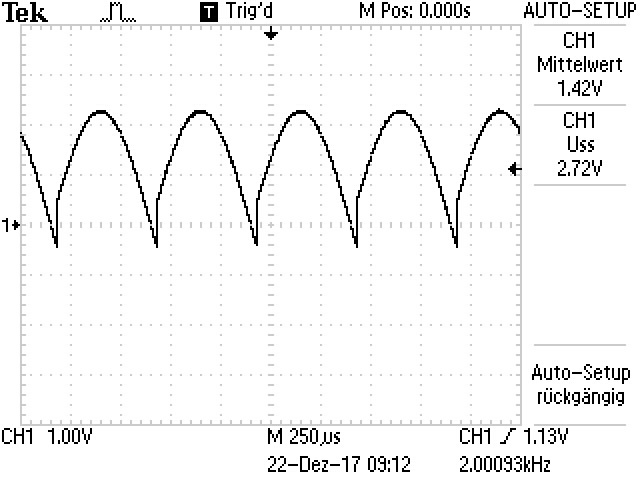
\includegraphics[width=\textwidth]{0Grad.JPG}
  \subcaption{Phasendifferenz bei 0 Grad}
\end{subfigure}
\begin{subfigure}{0.48\textwidth}
  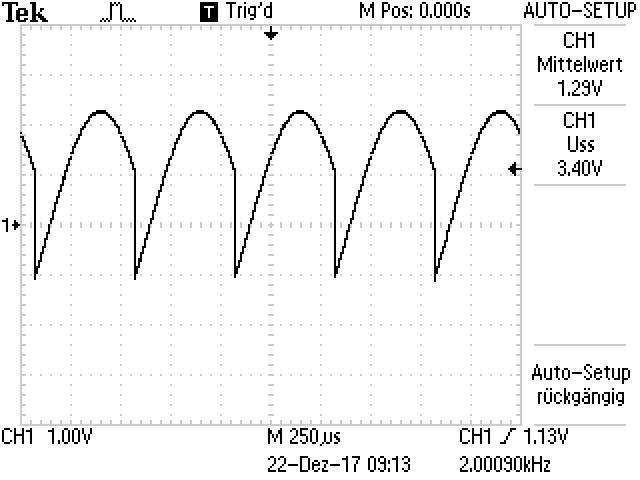
\includegraphics[width=\textwidth]{45Grad.JPG}
  \subcaption{Phasendiffernez bei 45 Grad}
\end{subfigure}
\begin{subfigure}{0.48\textwidth}
	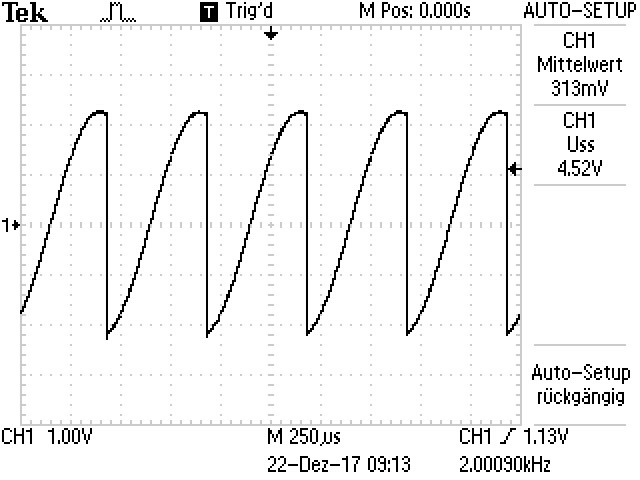
\includegraphics[width=\textwidth]{90Grad.JPG}
  \subcaption{Phasendifferenz bei 90 Grad}
\end{subfigure}
\begin{subfigure}{0.48\textwidth}
  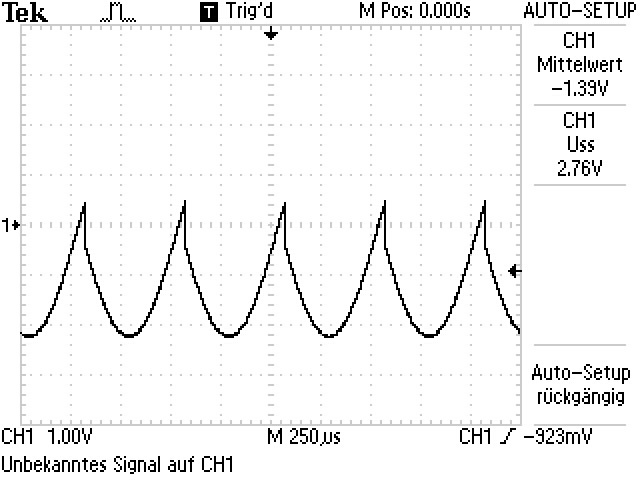
\includegraphics[width=\textwidth]{180Grad.JPG}
  \subcaption{Phasendiffernez bei 180 Grad}
\end{subfigure}
\begin{subfigure}{0.48\textwidth}
	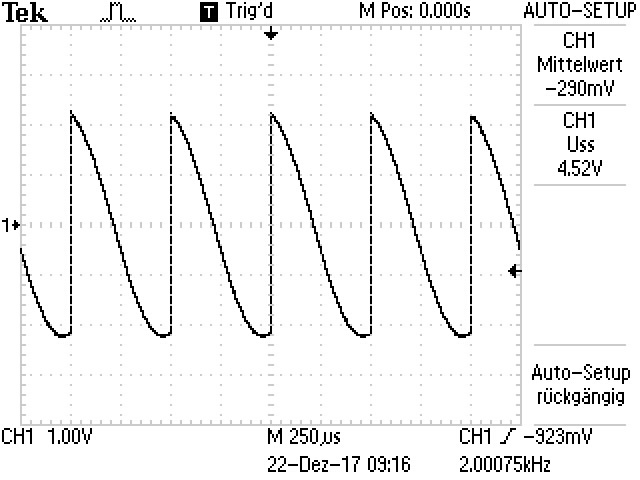
\includegraphics[width=\textwidth]{270Grad.JPG}
  \caption{Phasendifferenz bei 270 Grad}
\end{subfigure}
\end{figure}

Anschließend wird das Signal am Mischer durch ein Tiefpassfilter angeschlossen und folgende
Messwerte sind in der Tabelle (\ref{tab:1}) dargestellt.
\begin{table}[H]
\centering
\caption{Darstellung der Messergebnisse}
\label{tab:1}
 \begin{tabular}{c c c c}
  \toprule
     $U_\text{out} / V$ & $\Phi/\circ$ & $U_\text{theo} / V$ & $Abweichung / \%$ \\
  \midrule
  55,6  & 0   & 55,6  &??\\
  55,4  & 45  & 39,32 &??\\
  35,4  & 60  & 27,8  &??\\
  12,3  & 90  &   0   &??\\
  -19,4 & 120 &-27,8  &??\\
  -42,9 & 150 &-48,2  &??\\
  -55,3 & 180 &-55,6  &??\\
  -55,8 & 210 &-48,2  &??\\
  -37,3 & 240 &-27,8  &??\\
  -12,1 & 270 &   0   &??\\
  \bottomrule
\end{tabular}
\end{table}
Die Theoriewerte werden mit der Gleichung (5) berechnet. $U_o$ ist in diesem Fall durch den Vorverstärker
und Verstärker auf $87,34 V$ verstärkt worden.

Nun wird ein Rauschsignal hinzugeschaltet. Nun wird das Verfahren erneut durchgeführt.
Eine schematische Darstellung der Amplitude mit Rauschen in unterschiedlichen Phasen zeigt die nun folgenden
Bildschirmfotos dar.
\begin{figure}[H]
  \centering
  \begin{subfigure}{0.48\textwidth}
	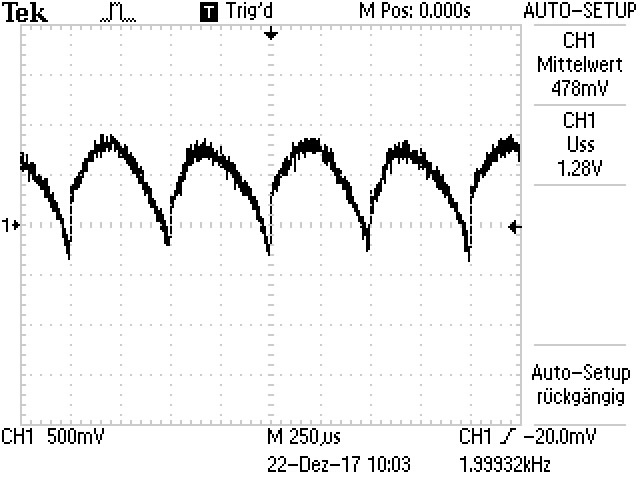
\includegraphics[width=\textwidth]{0GradR.JPG}
  \subcaption{Phasendifferenz bei 0 Grad}
\end{subfigure}
\begin{subfigure}{0.48\textwidth}
  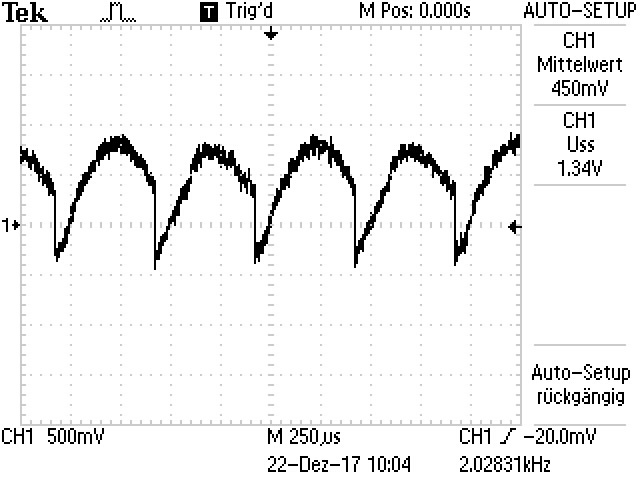
\includegraphics[width=\textwidth]{45GradR.JPG}
  \subcaption{Phasendiffernez bei 45 Grad}
\end{subfigure}
\begin{subfigure}{0.48\textwidth}
	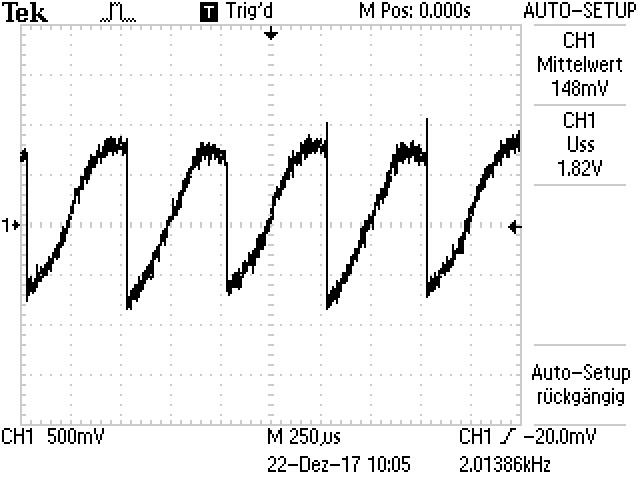
\includegraphics[width=\textwidth]{90GradR.JPG}
  \subcaption{Phasendifferenz bei 90 Grad}
\end{subfigure}
\begin{subfigure}{0.48\textwidth}
  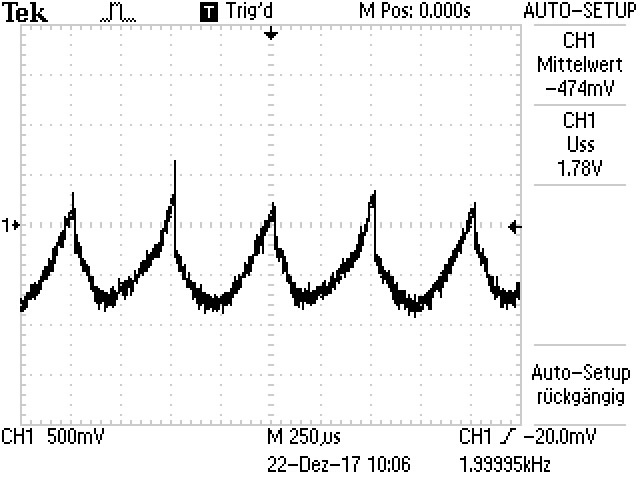
\includegraphics[width=\textwidth]{180GradR.JPG}
  \subcaption{Phasendiffernez bei 180 Grad}
\end{subfigure}
\begin{subfigure}{0.48\textwidth}
	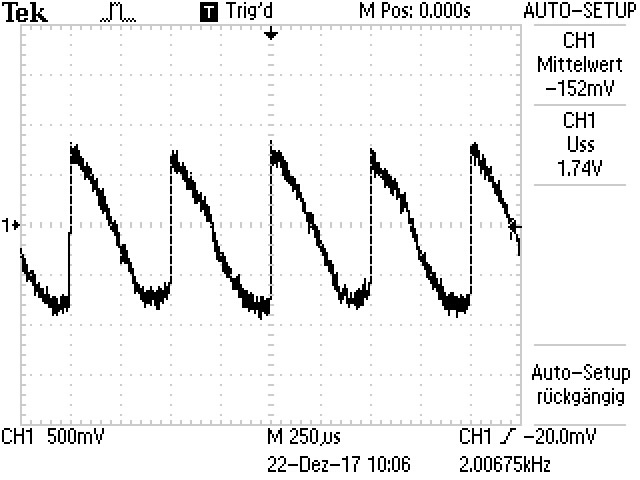
\includegraphics[width=\textwidth]{270GradR.JPG}
  \caption{Phasendifferenz bei 270 Grad}
\end{subfigure}
\end{figure}

Anschließend wird das Signal mit Rauschen am Mischer durch ein Tiefpassfilter angeschlossen und folgende
Messwerte sind in der Tabelle (\ref{tab:2}) dargestellt.
\begin{table}[H]
\centering
\caption{Darstellung der Messergebnisse für $U_o =87,34 V$}
\label{tab:2}
 \begin{tabular}{c c c c}
  \toprule
     $U_\text{out} / V$ & $\Phi/\circ$ & $U_\text{theo} / V$ & $Abweichung / \%$ \\
  \midrule
  49,2  & 0   & 55,6  &??\\
  49,6  & 45  & 39,32 &??\\
  33,8  & 60  & 27,8  &??\\
  14,6  & 90  &   0   &??\\
  -4,12 & 120 &-27,8  &??\\
  -36,7 & 150 &-48,2  &??\\
  -47,8 & 180 &-55,6  &??\\
  -49,6 & 210 &-48,2  &??\\
  -34,5 & 240 &-27,8  &??\\
  -14,6 & 270 &   0   &??\\
  \bottomrule
\end{tabular}
\end{table}


Bei der Leuchtdiode wird eine Rechteckspannung moduliert. Die eingestellte Frequenz ist $\omega = 159,6 \, \si{\hertz}$ und
besitzt eine Amplitude von $2 V$.
Folgende Messwerte werden in der Tabelle (\ref{tab:3}) dargestellt und in der Abbildung (\ref{abb:?}) als
Diagramm dargestellt.

\begin{table}[H]
\centering
\caption{Messreihe zur Leuchtdiode}
\label{tab:3}
 \begin{tabular}{c c| c c}
  \toprule
     $Intensität / V$ & $r / cm$ &  $Intensität / V$ & $r / cm$  \\
  \midrule
  4,19 & 2,5 & 2,08 & 30,5  \\
  4,44 & 3,5 & 1,84 & 32,5  \\
  4,71 & 4,5 & 1,44 & 37,5  \\
  4,98 & 5,5 & 1,14 & 42,5  \\
  5,28 & 6,5 & 1,03 & 47,5  \\
  5,55 & 7,5 & 0,82 & 52,5  \\
  5,68 & 8,5 & 0,73 & 57,5  \\
  5,92 & 9,5 & 0,66 & 62,5  \\
  6,20 & 10,5& 0,60 & 67,5  \\
  6,37 & 11,5& 0,56 & 72,5  \\
  6,55 & 12,5& 0,65 & 77,5  \\
  6,65 & 14,5& 0,54 & 82,5  \\
  6,15 & 16,5& 0,49 & 87,5  \\
  5,02 & 18,5& 0,44 & 92,5  \\
  4,24 & 20,5& 0,32 & 102,5 \\
  3,58 & 22,5& 0,27 & 112,5 \\
  3,06 & 24,5& 0,20 & 122,5 \\
  2,48 & 26,5& 0,16 & 132,5 \\
  2,32 & 28,5&   -  &  -    \\
  \bottomrule
\end{tabular}
\end{table}

\begin{figure}[H]
  \centering
	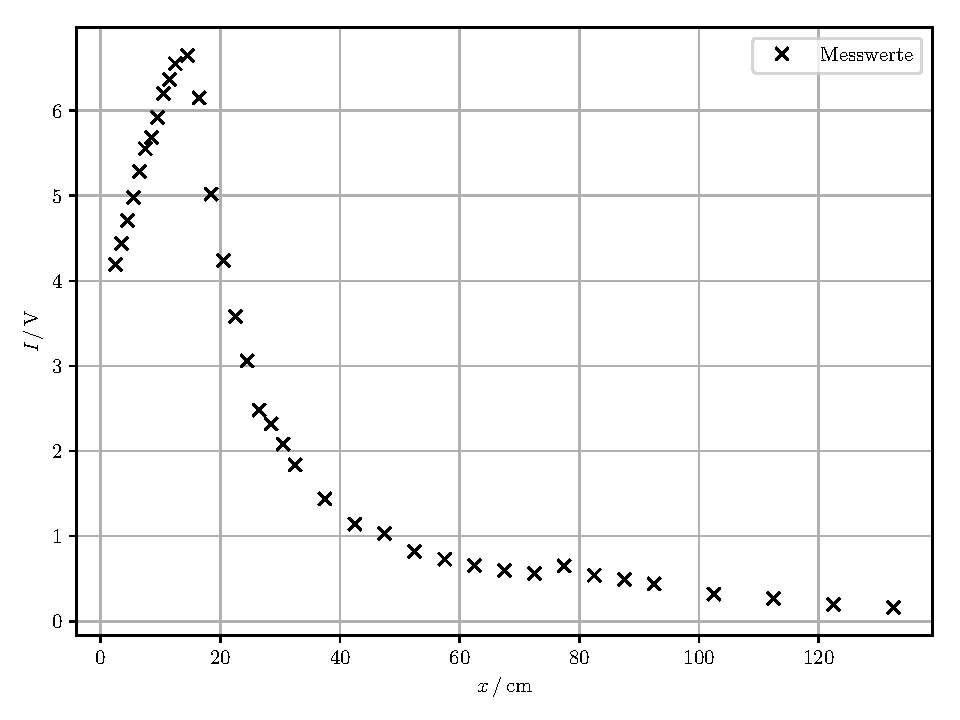
\includegraphics[width=\textwidth]{plot1.pdf}
  \caption{Darstellung der Intensität in Abhängigkeit des Abstandes}
  \label{abb:?}
\end{figure}

Die Werte bis zu dem Abstand $r = 14,5 cm$ sind physikalische nicht sinnvoll.
